
\chapter{Topic of this research}

Todo, Future Roland will have to write here...
The Research Chapter will need rework...
Read what is to be kept...
What should be removed...
etc...

This chapter establishes the research foundation for the project. It first presents the problem addressed and derives the research question. Based on this, the project's SMART goals are defined to provide clear guidance for the subsequent work. The chapter then identifies the research gap that motivates the project. Finally, core definitions related to data quality and data availability are introduced to provide the theoretical basis for the analysis and implementation presented in the following chapters.

Todo
Future Roland will have to rework this
Or at least review and restructure


\section{Problem statement}
\label{ResearchProblemState}

This work builds upon the previous research \cite{Roccaro2026_Project1}, which analysed the existing data pipelines at Swiss Post with regard to operational reporting. Based on this groundwork, the next logical step was to adapt the existing reports to the new reporting platforms. However, in the meantime, the reporting data pipelines were updated. The old data pipelines remained available, but all further updates were performed only on the new pipelines. As a result of this development, the focus of this project shifted towards supporting these changes and helping the team to improve the monitoring and assessment of the existing data. Furthermore, an important objective was to establish the groundwork for the upcoming master's thesis by evaluating whether the available tools could serve as the basis for a use case to be explored in greater depth during the thesis.





\subsection*{Problem generalisation}

This project bridges the groundwork established in the previous research towards the follow-up research in the master thesis. First, it has to perform the next step so that the stakeholders are able to continue checking their new data sources. Second, it must help to identify and test the tool for the master thesis. This is the most important part of the research, as it has to confirm that the selected tool is indeed a good match for the upcoming master thesis.



\section{Research gap}
\label{ResearchResearchGap}

Given this problem statement, the following questions are researched in more detail in the next two chapters. First, a theoretical introduction to the terms is provided; in later chapters, their specific meaning in the context of this project is discussed.



\section{High-level research question}
\label{ResearchResearchQuestion}

What is the next meaningful step to take in order to improve \gls{DA} and \gls{DQ} within the \gls{DWHLSOPS} team at Swiss Post? How can the business and IT be supported in achieving their objectives? While the solutions should be as simple as possible, they should be based on best practices and verified through scientific research. The research gap is addressed in the solution and implementation chapters. The main goal is to ensure that the conducted research provides tangible benefits to the team and contributes to future improvements. It is particularly important for the team that the research results are presented continuously so that progress, as well as potential deviations and changes, can be discussed.



\section{Success definition}
\label{ResearchSuccessDefinition}

The success criteria of this project are threefold and are defined based on the research gap as well as the initial project hand-in, which describes the business requirements.

First, the primary business objective is to achieve improvements through report updates. The goal of this project is to replace the existing report immediately and to establish concrete steps towards easier daily usage of the new report.

Second, communication with the business is another important success factor. The results from the research and implementation must be presented to the \gls{PO} on a regular basis.

Third, the testing and documentation of the basic setup required for the new DQM tool, as a theoretical and practical foundation for the master thesis, are the main achievements to be reached.



\section{S.M.A.R.T. Goals}
\label{ResearchSmartGoals}

The goals of this project are now defined here as “\gls{SmartGoals}”, as shown in the following list. They are all \textbf{S}pecific: the goal is clearly formulated; \textbf{M}easurable: there are measurable criteria defining when the goal is reached; \textbf{A}chievable: they are realistic given the available resources; \textbf{R}elevant: the goal is directly linked to the project’s success; and \textbf{T}ime-bound: there is a defined timeframe for achievement.

\begin{itemize}
\item \textbf{1) Setup of an Improved Data Quality Report}
    
\textbf{WHY:} This will help the team to run the daily checks faster.

By the end of the implementation phase, the existing data quality report is to be updated to use the new infrastructure. This includes new reporting data pipelines and the new structure using a star schema. Also, Power BI is to be used.

Success is measured by user feedback, which has to be obtained by the \gls{ASTV} team. The feedback is to be implemented, and the report must be on the production systems.

\item \textbf{2) Evaluation and Selection of DQM Platform for the Master Thesis}
    
\textbf{WHY:} To define the DQM platform for the master thesis.

During the implementation phase, the tool for the master thesis has to be defined. This requires a structured approach for the selection of the tool, including the setup of requirement lists. The team is to follow the DQM team during the evaluation of the tools.

Success is measured by having the DQM tool defined. The selected tool has to be discussed with the architect of the \gls{DWHLSOPS} team to make sure it fits the team's needs.

\item \textbf{3) Validation of the Selected DQM Tool}
    
\textbf{WHY:} The DQM platform must be tested for applicability to the master thesis.

By the end of the implementation phase, the DQM tool has to be tested for applicability to the master thesis. It must be proven that the required infrastructure can be set up for a test. Furthermore, a simplified test has to be run to confirm that the tool can handle the data sources.

Success is measured by having the DQM tool tested. The tool must return the test values to prove that it can be used for the follow-up master thesis.

\end{itemize}



\section{This project as a key step towards the “future state” reporting solution}
\label{SolutionIntentedSol}

As stated earlier the solutional goal of this project and its follow up is to provide an MVP for DQM, from which the key learnings will enable the full “future state” reporting solution. This MVP should implement an automatic data quality check, replacing an occasional, non automated check performed by the business. This is important, as the DQM check is currently executed by the business instead of IT, which creates challenges with regard to the desired target state. The expected situation would be that IT executes data quality checks and defines thresholds together with the business. At present, however, the knowledge about thresholds and other relevant information resides solely with the business.

In summary, having IT run the data checks would enable continuous follow-up of data quality. For example, a report based on automatically executed checks could show system uptime over a longer period of time. This information would later allow IT to extrapolate standard value ranges, which in turn would enable the definition of alerting thresholds. In short, having DQM checks executed automatically rather than occasionally by the business provides multiple benefits for both IT and the business.

\begin{figure}[H]
    \centering
    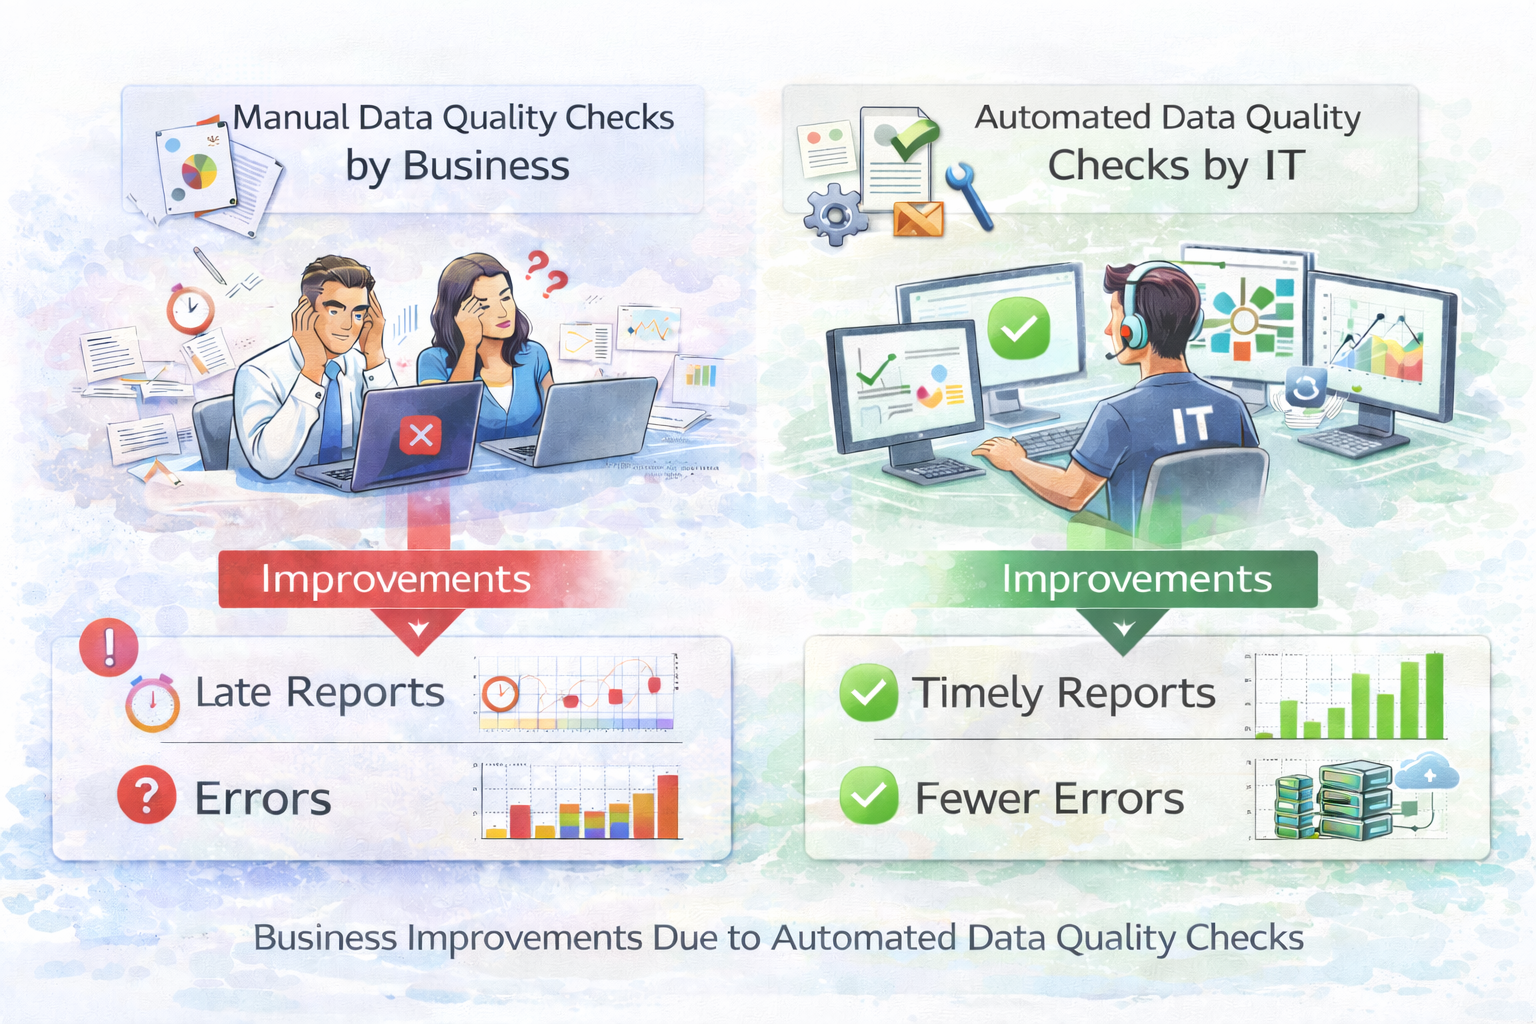
\includegraphics[width=0.8\textwidth]{./content/img/Solution_Design/businessChecks_against_ITautomated.png}
    \caption{DQM manual checks against automated checks by IT}
    \label{fig:dqm_manual_automated}
\end{figure}


\section{Expected benefits of this reporting solution}
\label{SolutionReasonsForSol}
A single visualisation does not explain the full benefit of the intended solution. For instance, the question arises as to why the business should stop performing data quality checks when it has the most detailed knowledge of the data. This is quickly clarified by taking a step back. The question should not be why checks are removed from the business, but why the reports are performed by the business in the first place. The benefits of this shift are therefore outlined in more detail in the following.

\subsection*{Benefit 1: Automation over manual processes to reduce effort}
\label{SolutionReasonsAutomationOverManual}
The business currently spends 30 to 45 minutes per day on a single data quality check, according to the initial project hand in description. From the duration of the check, it can be inferred that anyone requiring the data quality check before a report based on it is approved must wait until it is finished, resulting in a waiting time of 30 to 45 minutes. This fact provides the basis for understanding why manual processes are not suitable at scale. When scaling up to ten data quality checks, five to seven and a half hours are spent by the business on data quality checks. The waiting time for the last reports to be approved increases accordingly to five to seven and a half hours. When increasing to 20 checks per day, ten to 15 hours are spent, and the waiting time rises accordingly, accounting for more than one full-time position and long delays in report data release. It should be noted that this amount of time is spent solely to determine whether the defined check passes or not.
If the same initial check is executed by an automated data quality process, the expectation is that execution takes less than one minute; for simplicity, an execution time of one minute is assumed. As no manual initiation is required, no human time is spent performing the check. For comparison, the one minute waiting time for report approval and release is still considered. The business can then be informed whether the check returned an OK or not OK result, and the outcome can be stored for future reference.

When scaling this approach to ten checks, the total execution time remains ten times one minute. However, as the IT system can execute these checks in parallel, the waiting time for results remains at one minute. When increasing to 20 checks per day, the IT systems likewise execute the checks in parallel, and the execution and waiting time remain unchanged.

\subsubsection*{Benefit 2: Scalability to further reduce overall time required}
In summary, manual data quality checks cannot be scaled and lead to excessive use of human resources for repetitive tasks, as well as long waiting times for approved datasets. Automated data quality checks, by contrast, allow many checks to be executed in parallel within the same overall time frame. It should be noted that this comparison assumes all checks have similar complexity.

\subsection*{Benefit 3: Rule changes without query changes}
The current manual reports, which are business driven, have their logic built directly into the queries executed on the data. If any rule changes or a part of the data processing is modified, these queries need to be adapted. Thus, the check is deeply tied to the data source. To illustrate this with an example, a data quality check may confirm that 30\% of the data is category A and 70\% is category B, as this is considered the expected and valid distribution. If changes to processing pipelines or client behaviour cause the share of A to increase to 45\% and B to decrease to 55\%, the query performing the check must be adapted. However, when the check is performed by an application that injects these thresholds into a query, the query itself does not need to change, and only the parameters must be adjusted.

\subsubsection*{Benefit 4:  Reusability to improve stability and performance}
By moving the responsibility for checks from manual, business-driven processes to automated checks executed by IT, the checks can be designed to be more generic. Generic checks can be reused across different use cases. This separation of responsibilities and concerns leads to improved stability and performance when applying the checks, which in turn enables strong reusability. The same check type can be applied to different data sources by adapting parameters such as the query and thresholds, while the underlying check logic remains unchanged.




\section{Research Gap, Todo}

Todo
Work for future Roland


\section{Research Objective, Todo}

Todo
Work for future Roland



\section{Research Question, Todo}

Todo, Future Roland will have to write here...
The Research Chapter will need rework...
Read what is to be kept...
What should be removed...
etc...


\section{Research Hypotheses, Todo}
Todo, Future Roland will have to write here...
The Research Chapter will need rework...
Read what is to be kept...
What should be removed...
etc...


\section{Research Methodology, Todo}

Todo
Work for future Roland

\subsection{Research Approach, Todo}
\subsection{Comparison of Detection Approaches, Todo}
\subsection{Experimental Design, Todo}
\subsection{Evaluation Criteria and Metrics, Todo}



\section{Success Definition, Todo}

Todo, Future Roland will have to write here...
The Research Chapter will need rework...
Read what is to be kept...
What should be removed...
etc...


\section{S.M.A.R.T. Goals, Todo}

Todo
Work for future Roland


\section{Expected Contributions, Todo}

Todo
Work for future Roland
\subsection{Practical Contribution, Todo}
\subsection{Scientific Contribution, todo}


\section{Expected Benefits for the Reporting Solution, Todo}

Todo
Work for future Roland

 